%----------------------------------------------------------------------
% Harnessing cloud computing for high capacity analysis of neuroimaging
% data from NDAR
%
% Poster for OHBM 2015
%
% Contributing authors: Daniel Clark, Cameron Craddock
%----------------------------------------------------------------------

%----------------------------------------------------------------------
% Document class, packages, and formatting
%----------------------------------------------------------------------
\documentclass[final,hyperref={pdfpagelabels=false}]{beamer}

%% Packages
\usepackage{grffile}
\usepackage[english]{babel}
\usepackage[latin1]{inputenc}
\usepackage{amsmath,amsthm, amssymb, latexsym}
%\usepackage[framemethod=tikz]{mdframed}
%\usepackage{times}\usefonttheme{professionalfonts}  % obsolete
%\usefonttheme[onlymath]{serif}
%\boldmath
\usepackage{enumerate}
%\usepackage[orientation=portrait,size=custom,width=83.96,height=101,scale=1]{beamerposter}
\usepackage[orientation=portrait,size=custom,width=96,height=70,scale=1]{beamerposter}
%\usepackage[orientation=portrait,width=89,height=102,scale=1.1,debug]{beamerposter}
%\usepackage[orientation=portrait,size=a0,scale=1.4,debug]{beamerposter}
% change list indention level
% \setdefaultleftmargin{3em}{}{}{}{}{}
%\usepackage{snapshot} % will write a .dep file with all dependencies, allows for easy bundling

\usepackage{array,booktabs,tabularx}

%% Formatting
\mode<presentation>{\usetheme{CMINKI}}
\newcolumntype{Z}{>{\centering\arraybackslash}X} % centered tabularx columns
\newcommand{\pphantom}{\textcolor{ta3aluminium}} % phantom introduces a vertical space in p formatted table columns??!!
% Column sizing
\newlength{\columnheight}
\setlength{\columnheight}{72cm}

%\graphicspath{{figures/}}
\listfiles

%----------------------------------------------------------------------
% Title Block
%----------------------------------------------------------------------
%% Title
\title{\vskip1ex\Huge Harnessing cloud computing for high capacity analysis of neuroimaging data from NDAR}

%% Author
\author{\Large Daniel Clark$^1$, Christian Haselgrove$^2$, David Kennedy$^2$, Zhizhong Liu$^3$,\\[.5ex]Michael Milham$^1$, Petros Petrosyan$^4$, Carinna Torgerson$^3$, John Van Horn$^3$, Cameron Craddock$^1$}
\institute[NKI]{$^1$Child Mind Institute, New York, NY, $^2$ University of Massachuttes Medical School, Worcester, MA, $^3$University of Souther California, Los Angeles, CA, $^4$UCLA, Los Angeles, CA, $^5$Nathan S. Kline Institute for Psychiatric Research, Orangeburg, NY}

%% Poster info
\posternum{\Large 3535 Thursday 12:45}
\date[June 18th, 2015]{June 18th, 2015}

%----------------------------------------------------------------------
% Poster content
%----------------------------------------------------------------------
\begin{document}
\begin{frame}
    \begin{columns}
    % ---------------------------------------------------------%
    % Set up a column 
    \begin{column}{.5\textwidth}
      %\begin{beamercolorbox}[center,wd=\textwidth]{postercolumn}
        %\begin{minipage}[T]{.98\textwidth}  % tweaks the width, makes a new \textwidth
          \parbox[t][\columnheight]{\textwidth}{ % must be some better way to set the the height, width and textwidth simultaneously
            % Since all columns are the same length, it is all nice and tidy.  You have to get the height empirically
            %----------------------------------------------------------------------
            % Introduction
            %----------------------------------------------------------------------
            \begin{block}{Introduction}
              \begin{itemize}
                  \item The National Database for Autism Research (NDAR) hosts a vast collection of neuroimaging datasets that can be processed and utilized to yield significant scientific discoveries.
                  \item This amount of resources necessitates a high-performance computing (HPC) infrastructure, which is not always readily available for researchers in-house.
                  \item Amazon Web Services (AWS) Elastic Compute Cloud (EC2) computing service offers a ``pay as you go" model that allows researchers to utilize HPC performance without the up-front captial costs and maintenance of an in-house solution.
                  \item The developers of the Laboratory of Neuro Imaging (LONI) Pipeline, the Neuroimaging Informatics Tools and Resources Clearinghouse (NITRC) Computational Environment (CE) and the Configurable Pipeline for the Analysis of Connectomes (C-PAC) have implemented pipelines in EC2 that interface with NDAR
              \end{itemize}
            \vfill
            \end{block}
            %----------------------------------------------------------------------
            % Methods
            %----------------------------------------------------------------------
            \begin{block}{Methods}
                \vskip1ex
                \begin{column}{.47\textwidth}
                    \begin{figure}
                        \begin{center}
                            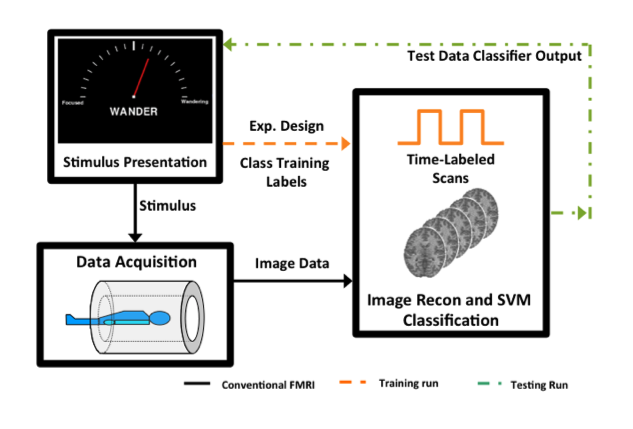
\includegraphics[width=.9\textwidth]{neurofeedback.eps}
                        \end{center}
                        \caption{\label{fig:roi_metrics}Neurofeedback experiment, adapted from S. LaConte$^{8,9}$}
                    \end{figure}
                \end{column}
                \begin{column}{.47\textwidth}
                {\bf Subjects} 
                \begin{itemize}
                  \item 13 volunteers participated in accordance with IRB Policy.
                \end{itemize}
                \vskip1ex
                
                {\bf Scanning}
                \begin{itemize}
                   \item 3.0T Siemens Magnetom TIM Trio using 12-channel head matrix.
                   \begin{itemize}
                      \item T1 weighted 3D MPRAGE anatomical scan (FA=8$^\circ$, TI=900ms, TR=2600ms, TE=3.02ms, GRAPPA $\times2$)
                      \item Realtime fMRI experiments were performed using an EPI seqeunce that has been customised to export
                        reconstructed image volumes, over a network connection, as they are connected$^{8,9}$
                      \begin{itemize}
                          \item TR/TE/FA/FOV = 2000 ms/30 ms/90$^\circ$/220 mm, in plane resolution 3.44 $\times$ 3.44 $\times$ 4 mm$^3$
                      \end{itemize}
                   \end{itemize}
                   \vskip1ex
                \end{itemize}
                \end{column}
                \vskip1ex
                
                \begin{column}{.48\textwidth}
                {\bf Online Preprocessing}
                \begin{itemize}
                    \item RT denoising implemented in AFNI$^{10}$ to remove contributions of confounds (intensity modulations induced by head motion, physiological noise, scanner drift, \dots)
                    \begin{itemize}
                        \item $N^{th}$ order polynomial
                        \item Global mean
                        \item Mask average time series (i.e. WM, CSF)
                        \item Motion parameters (6 or 24 regressor models)
                        \item Spatial smoothing
                    \end{itemize}
                   \item Adds $<$ 5 ms of delay
                \end{itemize}
                \end{column}
                \begin{column}{.50\textwidth}
                    \begin{figure}
                        \begin{center}
                            \includegraphics[width=.9\textwidth]{afni_denoise.eps}
                        \end{center}
                        \caption{\label{fig:afni_denoise}AFNI interface for online denoising.}
                    \end{figure}
                \end{column}
            \begin{figure}
                \begin{center}
                    \includegraphics[width=.60\textwidth]{flow_chart.eps}
                \end{center}
                \caption{\label{fig:processingflow}Flow chart of neurofeedback experiment.}
            \end{figure}    
            \vfill              
            \end{block}
          }
        %\end{minipage}
      %\end{beamercolorbox}
    \end{column}
    % ---------------------------------------------------------%
    % end the column

    % ---------------------------------------------------------%
    % Set up a column 
    \begin{column}{.5\textwidth}
      %\begin{beamercolorbox}[center,wd=\textwidth]{postercolumn}
       % \begin{minipage}[T]{.98\textwidth} % tweaks the width, makes a new \textwidth
          \parbox[t][\columnheight]{\textwidth}{ % must be some better way to set the the height, width and textwidth simultaneously
            % Since all columns are the same length, it is all nice and tidy.  You have to get the height empirically
            % ---------------------------------------------------------%
            % fill each column with content
            \begin{block}{Results}
              \begin{column}{.47\textwidth}
                  \begin{figure}
                      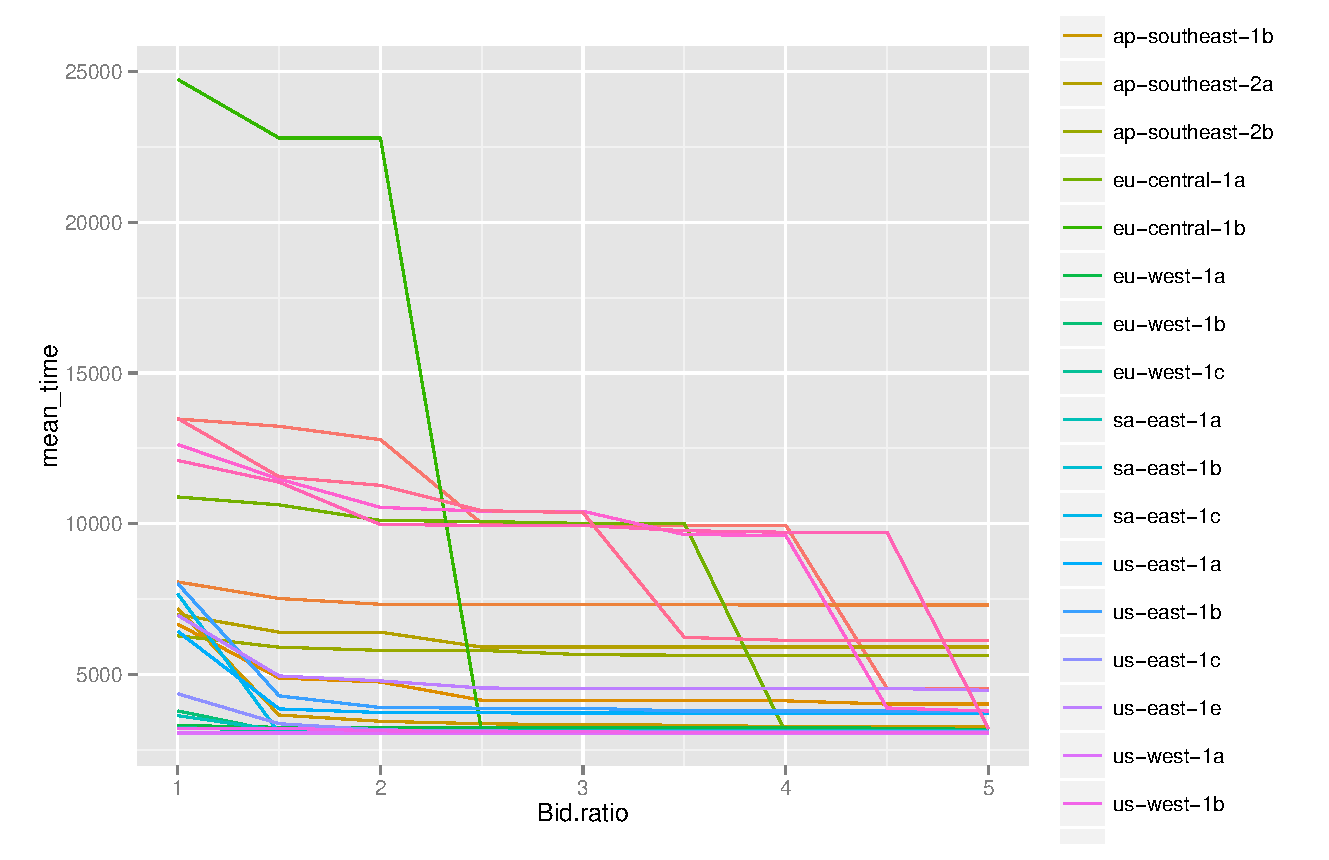
\includegraphics[width=.99\textwidth]{br_vs_time_fs.eps}
                      \caption{\label{fig:best_worst}Bid ratio vs Computation time in minutes for the Freesurfer pipeline}
                  \end{figure}
                  \vskip2ex
                  \begin{figure}
                      \includegraphics[width=.99\textwidth]{inter_subject.eps}
                      \caption{\label{fig:inter_subject} Performance across particpants (A) differs between feedback and neurofeedback scans as determined by their order (B).}
                  \end{figure}
                  \end{column}
                  \begin{column}{.49\textwidth}
                      \vskip4ex
                  \begin{figure}
                      \includegraphics[width=.99\textwidth]{beh_correlates.eps}
                      \caption{\label{fig:beh_correlates} Inter-individual variation in preformance correlates with behavioral measures.}
                  \end{figure}
              
                  \begin{itemize}
                       \item As shown in figure \ref{fig:best_worst} models learned for the best and worst performing participants match
                             with the canonical pattern of the default network.
                       \item The best participant was able to follow the instructures very well \ref{fig:best_worst}, the worst seems
                             to have been corrupted by noise.
                       \item Figure \ref{fig:inter_subject} shows 12 of the subjects were able to modulate the DN at above chance levels,
                             performance on feedback runs is consistent independent of order, but performance on nonfeedback runs improves
                             if they occur after feedback runs.
                       \item Measures that were significantly associated with DN regulation include ($p<0.05$, FDR corrected):  the affect intensity measure (AIM), ruminative responses scale (RRS), and the imaginal processes inventory. 
                  \end{itemize}
              \end{column}
            \end{block}
            \begin{block}{Conclusion}
              \begin{itemize}
                   \item We developed a system for measuring DN regulation using realtime neurofeedback. 
                   \item Participants were able to modulate their DN activity and their ability to do so was correlated with phenotype. 
                   \item This system provides a new experimental paradigm for understanding network dysregulation and how it maps to 
                        disease states and phenotype.
                   
                   
              \end{itemize}
            \end{block}
            \begin{block}{References and Acknowledgements}
                    1. Sonuga-Barke, E. et al. (2007), Neuroscience and Biobehavioral Reviews 31:977-986.\\
                    2. Broyd, S. J. et al. (2009), Neuroscience and Biobehavioral Reviews 33: 279-296.\\
                    3. Sheline, Y.I. et al. (2009), PNAS 106: 1942-1947.\\
                    4. Whitfield-Gabrieli, S. et al. (2009), PNAS 106: 1279-1284.\\
                    5. Hamilton, J.P. et al. (2011), Biol. Psychiatry 70: 327-333.\\
                    6. Sylvester, C.M. et al. (2012), Trends Neurosci. 35, 527-535.\\
                    7. Castellanos, F.X. et al. (2012), Trends Cogn. Sci. 16, 17-26.\\
                    8. LaConte, S.M. et al. (2004). Human Brain Mapping, 11: 2551.\\
                    9. LaConte, S.M. et al. (2011). NeuroImage, 56(2), 440-454.\\
                    10. Cox, R.W. (1996) Comput. Biomed. Res. 29: 162-173.\\
                    \vskip1ex
               Data collection and salary support was provided by a NARSAD Young Investigator Award to RCC.
             \end{block}
          }
          % ---------------------------------------------------------%
          % end the column
      %  \end{minipage}
      %\end{beamercolorbox}
    \end{column}
    % ---------------------------------------------------------%
    % end the column
  \end{columns}
\end{frame}
\end{document}


%%%%%%%%%%%%%%%%%%%%%%%%%%%%%%%%%%%%%%%%%%%%%%%%%%%%%%%%%%%%%%%%%%%%%%%%%%%%%%%%%%%%%%%%%%%%%%%%%%%%
%%% Local Variables: 
%%% mode: latex
%%% TeX-PDF-mode: t
%%% End:
